% TODO:
% - Add retail dataset results and description
% - !!! KDD reviews: several methods for generating the positive samples and negative samples, however, all of them are heuristic. It would be better if there are some principled methods or analysis
% - KDD reviews: authors should provide mathematical definitions of sequence and the task of learning embeddings in Section 3.1 and move the detailed introduction of the specific dataset to the experiment section. And there are many cases like this, so this paper needs further polish to improve the presentation.
% - KDD reviews: This work is on "lifestream" data. But I cannot see how it differs from the regular event sequences.
% - KDD reviews: the proposed method is "self-supervised" but does not justify the "self-supervision"
% - More links to respectful self-supervision theme is key in AI (for example key note from ICLR with Le Cun and Bendgio)
% - Add sampling motivation and no intersection of subsequences motivation (or delete that topic?)
% - Describe fine-tuning? (supplimentary material)
% - CPC vs MeLES picture
% - Make Tables with hyper-params experiment results more consistent

% DONE
% + Add games dataset results and description
% + Describe hand-crafted features? (supplementary material)
% + Add motivation of loss choice, find a paper where many losses was used and we took top 3.
% + Add description how CPC was adopted for event sequences.
% + Add: Metric learning in self-supervised manner was adopted for CV, not for event sequences.




\documentclass{article}
\usepackage[preprint, nonatbib]{neurips_2020}

\usepackage[utf8]{inputenc}
\usepackage[T1]{fontenc}
\usepackage{amsfonts}
\usepackage{microtype}
\usepackage{hyperref}

\usepackage{booktabs}
\usepackage{graphicx}
\usepackage[square,numbers]{natbib}
\usepackage{makecell}
\usepackage[ruled,vlined]{algorithm2e}
\usepackage{subcaption}

\title{MeLES: Metric learning for event sequences with self-supervision}

\author{
Dmitrii Babaev \thanks{D. Babaev, N. Ovsov and I. Kireev contributed equally to this work.} \\
% dmitri.babaev@gmail.com
Sberbank AI Lab
\And
Ivan Kireev \\
Sberbank AI Lab
\And
Nikita Ovsov \\
Sberbank AI Lab
\And
Maria Ivanova \\
Sberbank AI Lab
\And
Gleb Gusev \\
Sberbank AI Lab
\And
Alexander Tuzhilin \\
% atuzhili@stern.nyu.edu
New York University
}

\newcommand{\nt}[1]{{\bf [#1]}}

\begin{document}

\maketitle

\begin{abstract}

In our research we address the problem of learning representations for discrete event sequences generated by real-world users.

Constructing semantically meaningful embeddings from a huge amount of unlabelled data generated by real-world users is a challenging representation learning problem. Those pre-trained embeddings incorporate complex information from the raw discrete data as low-dimensional fixed-length vectors and could be easily applied in various downstream machine learning tasks as features or fine-tuned for specific target. In this paper we propose a novel method: Metric Learning for Event Sequences (MeLES), used to obtain lifestream data representation in the latent space. Traditionally, metric learning approach requires pairs of objects labeled as the same, but those pairs are often not available for lifestream data. So we propose a strategy based on sub-sequences generation from the raw data motivated by its periodicity and repeatability.

We evaluated MeLES over several public bank transactions datasets and showed that self-supervised embeddings outperform other methods when applied to downstream classification tasks. Moreover, embeddings are compact and provide additional user privacy protection.

\end{abstract}

\section{Introduction} \label{sec-intro}

The size of the dataset is of prime significance for the modeling quality for many supervised learning tasks~\cite{Sun2017RevisitingUE}. However, for many real word scenarios it is not possible to gather enough labeled data. This problem motivated extensive research in the area of knowledge transfer where the model trained for some task can be used as a good staring point for training for another task. The approach known as self-supervised learning is to define a synthetic task encouraging exploration of the internal structure of the data. Self-supervised learning is the natural option for pre-training in situations when there is no large enough labelled dataset for the task of interest or for a similar task.

Self-supervised learning has demonstrated effectiveness in different machine learning domains, including that of Natural Language Processing, e. g. ELMO~\cite{Peters2018DeepCW}, BERT~\cite{Devlin2019BERTPO}) and computer vision~\cite{Doersch2015UnsupervisedVR}. There are also specialized methods that apply self-learning to non-discrete sequences, such as CPC~\cite{Oord2018RepresentationLW}. However, there has been very little work on how to apply this techniques to other domains including the domain of discrete event sequences. One common example of discrete event sequences is user behavior sequences~\cite{Ni2018PerceiveYU}, the discrete event sequences generated by real-world users. User behavior sequences is produced in many business applications, some examples being credit card transactions and click-stream data of internet site visits, and their analysis constitutes a very common machine learning problem~\cite{Laxman2008StreamPU, Wiese2009CreditCT, Zhang2017CreditRA, Bigon2019PredictionIV}. User behavior sequence is an event sequence that is attributed to a person and captures his/her regular and routine actions of certain type, e.g., transactions, search queries, phone calls and messages.


In this paper, we propose the \emph{Metric Learning for Event Sequences (MeLES)} method that learns low-dimensional representations of discrete event sequences. This is the first method designed specifically for the discrete event sequences which copes with specific properties of that type of data by 
% In a broad sense, MeLES method 
adopting metric learning techniques~\cite{Xing2002DistanceML, Hadsell2006DimensionalityRB}. Metric learning is often used in a supervised manner for mapping high-dimensional objects to a low-dimensional embedding space. The aim of metric learning is to represent semantically similar objects (images, video, audio, etc.) closer to each other, while dissimilar ones further away. Most of the metric learning methods are used in such applications as speech recognition~\cite{Wan2018GeneralizedEL}, computer vision~\cite{Schroff2015FaceNetAU, Mao2019MetricLF} and text analysis~\cite{Reimers2019SentenceBERTSE}. In these domains, metric learning is successfully applied in a supervised manner to datasets, where pairs of high-dimensional instances are labeled as the same object or different ones.
MeLES is based on the observation that often property of an event sequence is periodicity and repeatability of events. Therefore, one can consider some convenient sub-sequences of the same sequence as auxiliary high-dimensional representations of the same stochastic process that produced the observed sequence. By utilizing sub-sequence generation, it is possible to combine metric learning with self-supervision and get an algorithm that does not require labelling.
MeLES model trained in a self-supervised manner can be used in two ways. Representations, produced by the model can be directly used as a fixed vector of features in some supervised downstream task (e. g. classification task) similarly to~\cite{Mikolov2013EfficientEO, Song2017LearningUE, Zhai2019LearningAU}. Alternatively, trained model can be fine-tuned~\cite{Devlin2019BERTPO} for the specific downstream task.

We conducted experiments on several different user behavior sequence~\cite{Ni2018PerceiveYU} datasets and evaluated performance of the method on downstream classification tasks. When MeLES representations is directly used as features, the method achieves strong performance comparable to the baseline methods. The fine-tuned representations achieve the state-of-the-art performance on downsteam classification tasks, outperforming several other supervised methods and methods with unsupervised pre-training by a significant margin. Moreover, we show superiority of MeLES embeddings over the supervised approach applied to the partially labeled raw data due to insufficient amount of the target to learn a sufficiently complex model from scratch.

In this paper, we make the following contributions. We
\begin{enumerate}
    \item adopted the ideas of metric learning to the analysis of the discrete event sequences in a novel self-supervised manner;
    \item proposed a specific method, called Metric Learning for Event Sequences (MeLES), to accomplish this task;
    \item demonstrated that the proposed MeLES method significantly outperforms other baselines for both the supervised and the semi-supervised learning scenarios on several different user behavior sequence~\cite{Ni2018PerceiveYU} datasets.
\end{enumerate}

We provide the full source code for all the experiments described in the paper\footnote{https://github.com/***/*** (the link was anonymized for the double-blind peer review purposes)}.


\section{MeLES method} \label{sec-method}

\nt{Here should be a short introduction to the problem and short description of what are discrete event sequences. Here is a bad draft.} Given a sequence of discrete events $\{x_t \}^T_{t=1}$ in a given observation interval $[1, T]$, our goal is to represent it, in a self-supervised manner, in a latent space $R^d$ by its meaningful embedding $c$, which encodes information about the entity associated with the sequence and filters out stochastic aspects of the sequence. This embedding should be useful for different downstream tasks abut the entity. In this paper, we propose MeLES, a novel concept, which enables to introduce ideas of metric learning into this self-supervised setting.

Metric learning methods were initially developed for supervised tasks, where some (\textit{positive}) pairs of examples are labeled as the same entity (or similar), while some (\textit{negative}) pairs are labeled as different (dissimilar) ones.

We describe the idea of metric learning using a specific formalism that we further apply to our setting. Metric learning has applications in different domains (CV, speech, NLP, etc.), where the same \textit{person} or \textit{entity} can be represented by different \textit{samples} 
\nt{or "specimens"?}. We assume that each entity $e$ is associated with a probabilistic distribution $P_e$ over all possible samples (e.g., a person is a distribution over all his/her pictures that can potentially appear in the life). A mapping $M$ \nt{refer} that we learn defines a pushforward $P_M(e):=M\#P_e$ of this distribution in the feature space \nt{refer}. The idea of metric learning (samples of the same entity represented in the feature space should be closer to each other than samples of different entities) can be rephrased as follows: distributions $P_M(e)$ of different entities $e$ should be separated in the latent space as much as possible. The aim of previous literature on metric learning is to identify the entity based on its sample \nt{references}. Therefore, their training datasets naturally contain several independent samples per each particular entity, which form~\textit{positive pairs} (pairs of samples of the same entity) as a critical component for learning.

On the contrary, our aim is a novel self-supervised approach to representation learning intended for a wide range of tasks with sequential data, and we have no positive pairs. Instead, we have only one sequence per one entity (one sequence of transactions for a client, one click log for a user, and so on). According to the above formalism, each entity $e$ is associated with a distribution over event sequences, i.e., with a latent stochastic process $\{X_e(t)\}$. \nt{Something about the range of $t$.} In this way, particular event sequence $\{x_e(t)\}$ that represents entity $e$ in our event sequence data is generated by this process $\{X_e(t)\}$.

MeLES samples positive pairs as sub-sequences of the same person sequence and negative pairs as sub-sequences from different person sequences. See section \ref{sec-pos-pairs} for details of the positive pairs generation.

\nt{About applicability of MeLES to different domains.}

\nt{This paragraph should be revised.}
Embedding $c_t$ is generated by encoder neural network which is described in section~\ref{sec-enc-arch}. Metric learning losses are described in section \ref{sec-ml-loss}. Positive pairs generation strategies are described in section \ref{sec-pos-pairs}. Negative pairs sampling strategies are described in section \ref{sec-neg-samples}. 


\subsection{Sampling of surrogate sequences} \label{sec-pos-pairs}

If we had pairs of sample sequences generated by the same process $\{X_e(t)\}$, we could apply metric learning to our task. While we have no access to the latent process $\{X_e(t)\}$, we hope to generate \textit{surrogate} sequences as sub-sequences of the same event sequence $\{x_e(t)\}$ instead. The idea proposed below resembles the bootstrap method~\cite{Efron1994Bootstrap}, which enables to generate several bootstrap samples using only one sample of independent datapoints of a latent distribution. However, our setting is different, since we have no independent observations, so we should rely on different data assumptions.

The key property of event sequences that represent life activity is periodicity and repeatability of the events in the steam. This observation is a motivation for the \textit{Random slices} sampling method applied for MeLES, see Algorithm~\ref{alg-slce-ss}. Each sub--sequence is generated from the initial sequence as its connected segment ("slice") in two steps. First, the length of the slice is chosen uniformly from possible values. Second, its starting position is uniformly chosen from all possible values.

\begin{algorithm}
\SetAlgoLined
\textbf{hyperparameters:} $m, M$: minimal and maximal possible length of sub-sequence\\ $k$: number of sub-sequences to be produced. \\
\textbf{input:} A sequence $S$ of length $l$. \\
\textbf{output:} $S_1,...,S_k$: sub-sequences of $S$. \\

\BlankLine
 \For{$i\leftarrow 1$ \KwTo $k$}{
 Generate random integer $l_i$ from $[m, \min(M,l)].$\\
 Generate random integer $s$ from $[0, l-l_i].$\\
 $S_i = S[s: s + l_i]$
 }
 
\caption{Random slices sub-sample generation strategy}
\label{alg-slce-ss}
\end{algorithm}

\subsection{Theoretical analysis}

Assume that length $T$ of observed sequence $x_e(t)$ follows a power--law distribution.


\subsection{General framework}

\begin{figure}[htbp]
  \caption{General framework}
  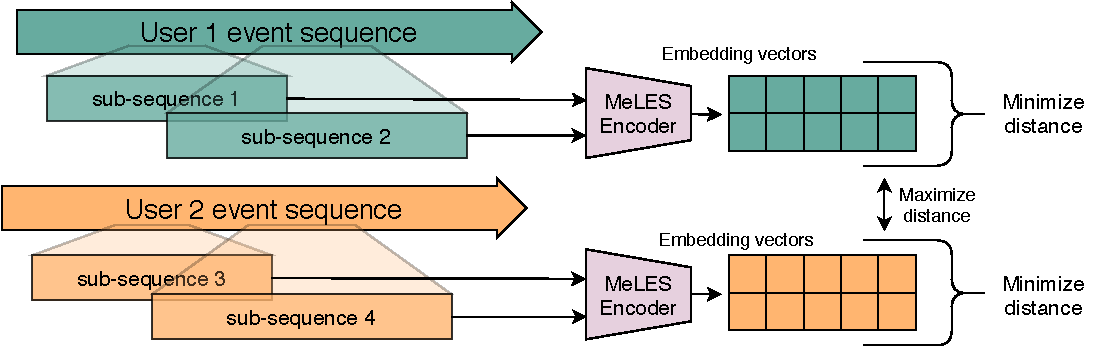
\includegraphics[width=\linewidth]{figures/arch-v2-narrow.pdf}
  \label{fig-arch}
\end{figure}

The overview of the method is presented in Figure \ref{fig-arch}.


One of the difficulties with applying metric learning approach to the discreet event sequeinces is that the notion of semantic similarity as well as dissimilarity requires underlying domain knowledge and human labor-intensive labeling process to constrain positive and negative examples. 


Sequence embedding $c_t$ obtained by the metric learning approach is then used in various donwstream machine learning tasks as a feature vector. Also, a possible way to improve the downstream task performance is to feed a pre-trained embedding $c_t$ (e. g. the last layer of RNN) to a task-specific classification subnetwork and then jointly fine-tune the model parameters of the encoder and classifier subnetworks.


\subsection{Metric learning losses} \label{sec-ml-loss}

Metric learning loss discriminates embeddings in a way that embeddings from same class are moved closer together and embeddings from the different class are moved further. We have considered several metric learning losses that showed promising performance on the different datasets~\cite{Kaya2019DeepML} and also some classical variants, namely, contrastive~loss~\cite{Hadsell2006DimensionalityRB}, binomial deviance loss~\cite{Yi2014DeepML}, triplet loss \cite{Hoffer2015DeepML}, histogram~loss~\cite{Ustinova2016LearningDE} and margin~loss~\cite{Manmatha2017SamplingMI}.

Contrastive loss is conceptually simple, and yet demonstrated strong performance on validation set in our experiments (see Table \ref{tab-loss-type}), namely contrastive loss and margin loss.
Contrastive loss has a contrastive term for the negative pair of embeddings which penalizes the model only if the negative pair is not distant enough and the distance between embeddings is less than a margin $m$:  
\begin{equation}
 \mathcal{L} = \sum_{i=1}^P \left[ (1-Y)\frac{1}{2}(D_W^i)^2 +Y*\frac{1}{2}\{max(0,m-D_W^i)\}^2 \right],
\end{equation}
where $P$ is the count of all pairs in a batch, $D_W^i$ - is a distance function between an i-th labeled sample pair of embeddings $X_1$ and $X_2$, 
$Y$ is a binary label assigned to a pair: $Y = 0$ means a similar pair, $Y = 1$ means dissimilar pair, $m > 0$ is a margin.
As proposed in~\cite{Hadsell2006DimensionalityRB} we use euclidean distance as the distance function: $D_W^i = D(A,B) = \sqrt{\sum_i(A_i - B_i)^2}$.

\subsection{Batch generation}

The following procedure is used to create a batch during MeLES training. $N$ initial sequences are taken for batch generation. Then, $K$ sub-sequences are produced for each initial sequence.

Pairs of sub-sequences produced from the same sequence are considered as positive samples and pairs from different sequences are considered as negative samples. Hence, after positive pair generation each batch contains $N \times K$ sub-sequences used as training samples. There are $K-1$ positive pairs and $(N - 1) \times K$ negative pairs per sample in batch.

There are several possible strategies of sub-sequence generation. The simplest strategy is the random sampling without replacement. Another strategy is to produce a sub-sequence from random splitting sequence to several sub-sequences without intersection between them (see Algorithm \ref{alg-disj-ss}). The third option is to use randomly selected slices of events with possible intersection between slices (see Algorithm \ref{alg-slce-ss}). 

Note, that the order of events in generated sub-sequences is always preserved.

\begin{algorithm}
\SetAlgoLined
\textbf{hyperparameters:} $k$: number of sub-sequences to be produced. \\
\textbf{input:} A sequence $S$ of length $l$. \\
\textbf{output:} $S_1,...,S_k$: sub-sequences of $S$. \\

\BlankLine
Generate vector $inds$ of length $l$ with random integers from [1,k].\\
 \For{$i\leftarrow 1$ \KwTo $k$}{
 $S_i = S[inds == i]$
 }
\caption{Disjointed sub-sequences generation strategy}
\label{alg-disj-ss}

\end{algorithm}




\subsection{Hard negative sampling} \label{sec-neg-samples}

Negative sampling is a way to address the following challenge of the metric learning approach: using all pairs of samples is inefficient, for example, some of the negative pairs are already distant enough thus this pairs are not valuable for the training~\cite{SimoSerra2015DiscriminativeLO, Manmatha2017SamplingMI, Schroff2015FaceNetAU}. Hence, only part of possible negative pairs are considered during loss calculation. Note that only current batch samples are considered. There are several possible strategies of selecting most relevant negative pairs.

\begin{enumerate}
    \item Random sample of negative pairs
    \item Hard negative mining: generate k hardest negative pairs for each positive pair.
    \item Distance weighted sampling, where negative samples are drawn according to their relative distance from the anchor.~\cite{Manmatha2017SamplingMI}
    \item Semi-hard sampling, where we choose the nearest to anchor negative example, from samples which further away from the anchor than the positive exemplar~\cite{Schroff2015FaceNetAU}.
\end{enumerate}

In order to select negative samples, we need to compute pair-wise distance between all possible pairs of embedding vectors of a batch. For the purpose of making this procedure more computationally effective we perform normalization of the embedding vectors, i.e. project them on a hyper-sphere of unit radius. Since $D(A,B) = \sqrt{\sum_i(A_i - B_i)^2} = \sqrt{\sum_i A_i^2 + \sum_i B_i^2 - 2\sum_i A_i B_i} $ and $||A||= ||B||=1$, to compute the the euclidean distance we only need to compute: $\sqrt{2 - 2(A \cdot B)}$.

To compute the dot product between all pairs in a batch we just need to multiply the matrix of all embedding vectors of a batch by itself transposed, which is a highly optimized computational procedure in most modern deep learning frameworks. Hence, the computational complexity of the negative pair selection is $O(n^2h)$ where $h$ is the size of the output embeddings and $n$ is the size of the batch.

\subsection{Encoder architecture} \label{sec-enc-arch}

To embed a sequence of events to the fixed-size vector $c \in R^d$ we use approach similar to the E.T.-RNN card transaction encoder proposed in~\cite{Babaev2019ETRNNAD}. The whole encoder network consists of two conceptual parts: the event encoder and the sequence encoder subnetworks.

The event encoder $e$ takes the set of attributes of a single event $x_t$ and outputs its representation in the latent space $Z \in R^m$: $z_t = e(x_t)$. The sequence encoder $s$ takes latent representations of the sequence of events: $ z_{1:T} = z_1, z_2, \cdots z_T $ and outputs the representation of the whole sequence $c_t$ in the time-step $t$: $ c_t = s(z_{1:t}) $.

The event encoder consists of the several embedding layers and batch normalization~\cite{Babaev2019ETRNNAD} layer. Each embedding layer is used to encode each categorical attribute of the event. Batch normalization is applied to numerical attributes of the event. Finally, outputs of every embedding layer and batch normalization layer are concatenated to produce the latent representation $z_t$ of the single event.

The sequence of latent representations of event representations $z_{1:t}$ is passed to sequence encoder $s$ to obtain a fixed-size vector $c_t$. Several approaches can be used to encode a sequence. One possible approach is to use the recurrent network (RNN) as in~\cite{Sutskever2014SequenceTS}. The other approach is to use the encoder part of the Transformer architecture presented in~\cite{Vaswani2017AttentionIA}. In both cases the output produced for the last event can be used to represent the whole sequence of events. In case of RNN the last output $h_t$ is a representation of the sequence.

Encoder, based on RNN-type architecture like GRU~\cite{Cho2014LearningPR}, allows to calculate embedding $c_{t+k}$ by updating embedding $c_t$ instead of  calculating embedding $c_{t+k}$ from the whole sequence of past events $z_{1:t}$: $c_k = rnn(c_t, z_{t+1:k})$. This option allows to reduce inference time to update already existing person embeddings with new events, occurred after the calculation of embeddings. This is possible due to the recurrent nature of RNN-like networks.



\section{Experiments} \label{sec-exp}

\subsection{Datasets} \label{sec-datasets}

In our research we used several publicly available datasets of bank transactions.
\begin{enumerate}
    \item \textbf{Age group prediction competition}\footnote{https://onti.ai-academy.ru/competition} - the dataset of 44M anonymized transactions representing 50k persons was used to predict the age group of a person. Each transaction includes date, type and amount.
        
    \item \textbf{Prediction of client gender on card transactions}\footnote{https://www.kaggle.com/c/python-and-analyze-data-final-project/} - the dataset of 6,8M anonymized card transactions representing 15k clients was used to predict a gender. Each transaction is characterized by date, type, amount and Merchant Category Code.
    
    \item \textbf{Data Science Bowl}\footnote{https://www.kaggle.com/c/data-science-bowl-2019} - the task is to predict the in-game assessment results based on the history of children gameplay data. The dataset consists of 12M gameplay events representing 4,6k children. Each gameplay event is characterized by timestamp, event code, incremental counter of events within a game session, time since the start of the game session, etc.
    
    \item \textbf{Gender prediction competition}\footnote{https://ods.ai/competitions/x5-retailhero-uplift-modeling} - the task is to predict the age group of a client based on it retail purchase history. The dataset consists of 45,8M retail purchases representing 400k clients. Each purchase is characterized by time, product level, segment, amount, value, points received.
    
    
    
    
\end{enumerate}

This particular publicly available datasets were chosen for sufficient amount of complex discrete events per user, hence, suitable for our method to obtain meaningful representations. 

We selected the this particular datasets and predication because of the public availabily, richness, large volume of data ... The demography prediction tasks are popular in the marketing domain, e. g. both Google and Facebook Ad management consoles allows to target Ads to the specific demographic groups.

\subsection{Experiment setup}

For each dataset, we set apart 10\% persons from the labeled part of data as the test set that we used for comparing different models.
For all methods random search on 5-fold cross-validation over the train set is used for hyper-parameter selection. The hyper-parameters with the best out-of-fold performance on train set is then chosen.
For evaluation of semi-supervised/self-supervised techniques (including MeLES), we used all transactions including unlabeled data, except for the test set, as far as those methods are suitable for partially labeled datasets, or does not require labels at all.

\subsubsection{Performance}

Neural network training was performed on a single Tesla P-100 GPU card. For the training part of MeLES, the single training batch is processed in 142 millisecond. For age prediction dataset, the single training batch contains 64 unique persons with 5 sub-samples per person, i.e. 320 training samples in total, the mean number of transactions per sample is 90, hence each batch contains around 28800 transactions.

\subsubsection{Baselines} \label{sec-baselines}

We compare our MeLES method with the following two baselines. First, we consider the Gradient Boosting Machine (GBM) method~\cite{Friedman2001GreedyFA} on hand-crafted features. GBM can be considered as a strong baseline in cases of tabular data with heterogeneous features. In particular, GBM-based approaches achieve state-of-the-art results in a variety of practical tasks including web search, weather forecasting, fraud detection, and many others~\cite{Wu2009AdaptingBF, Vorobev2019LearningTS, Zhang2015AGB, Niu2019ACS}.

Second, we apply recently proposed Contrastive Predictive Coding (CPC)~\cite{Oord2018RepresentationLW}, a self-supervised learning method, which has shown an excellent performance for sequential data of such traditional domains as audio, computer vision, natural language, and reinforcement learning. We adopted CPC for discrete event sequences; the model task is to distinguish true future event from other event using series of previous events as an input.

GBM based model requires a large number of hand-crafted aggregate features produced from the raw transactional data. An example of an aggregate feature would be an average spending amount in some category of merchants, such as hotels of the entire transaction history.
We used LightGBM~\cite{Ke2017LightGBMAH} implementation of GBM algorithm with nearly 1k hand-crafted features for the application. Please see the companion code for the details of producing hand-crafted features.

In addition to the mentioned baselines we compare our method with supervised learning approach where the encoder sub-network and with classification sub-network are jointly trained on the downstream task target. Note, that no pre-training is used in this case.

\subsubsection{Design choices}

If we do not explicitly mention alternative, in our experiments we use contrastive loss and random slices pair generation strategy. We evaluated several possible loss choices and found that even contrastive loss that can be considered as the basic variant of metric learning loss allows to get strong results on the downstream tasks (see supplementary material, Table \ref{tab-loss-type}). Our hypothesis is that an increase in the model performance on metric learning task does not always lead to an increase in performance on downstream tasks.

Observe that hard negative mining leads to significant increase in quality on downstream tasks in comparison to random negative sampling (see Table \ref{tab-neg-sampl}).

Another observation is that a more complex sub-sequence generation strategy (e. g. random slices) shows slightly lower performance on the downstream tasks in comparison to the random sampling of events (see Table \ref{tab-pair-gen}).

The final set of hyper-parameters used for MeLES is shown in the supplementary material, Table \ref{sup-tab-hyper}.

\begin{table}
\centering
\caption{Comparison of pair generation strategies}
\begin{tabular}{llll}
\toprule
\textbf{Dataset} & \textbf{Random samples} & \textbf{Random disjoint samples} & \textbf{Random slices} \\
\midrule
\makecell{\textbf{Age group} \small{(Accuracy)}} & $0.628 \pm 0.003$ & $0.608 \pm 0.004$ & $0.639 \pm 0.006$ \\
\makecell{\textbf{Gender} \small{(AUROC)}} & $0.851 \pm 0.004$ & $0.836 \pm 0.008$ & $0.872 \pm 0.005$ \\
\makecell{\textbf{Attempts} \small{(Accuracy)}} & $0.546 \pm 0.004$ & $0.0 \pm 0.0$ & $0.604 \pm 0.003$ \\
\bottomrule
\end{tabular} \\
\small{5-fold cross-validation metric $\pm 95\%$ is shown}
\label{tab-pair-gen}
\end{table}

\begin{table}
\centering
\caption{Comparison of negative sampling strategies}
\begin{tabular}{llll}
\toprule
\textbf{Dataset} & \makecell{\textbf{Hard negative} \\ \textbf{mining}} & \makecell{\textbf{Random negative} \\ \textbf{sampling}} & \makecell{\textbf{Distance weighted} \\ \textbf{sampling}} \\
\midrule
\makecell{\textbf{Age group} \small{(Accuracy)}} & $0.637 \pm 0.005$ & $0.615 \pm 0.005$ & $0.620 \pm 0.003$ \\
\makecell{\textbf{Gender} \small{(AUROC)}} & $0.872 \pm 0.004$ & $0.826 \pm 0.004$ & $0.867 \pm 0.003$ \\
\makecell{\textbf{Attempts} \small{(Accuracy)}} & $0.604 \pm 0.003$ & $0.602 \pm 0.002$ & $0.604 \pm 0.001$ \\
\bottomrule
\end{tabular} \\
\small{5-fold cross-validation metric $\pm 95\%$ is shown}
\label{tab-neg-sampl}
\end{table}

\begin{figure}
  \centering
  \begin{minipage}[t]{0.49\linewidth}
    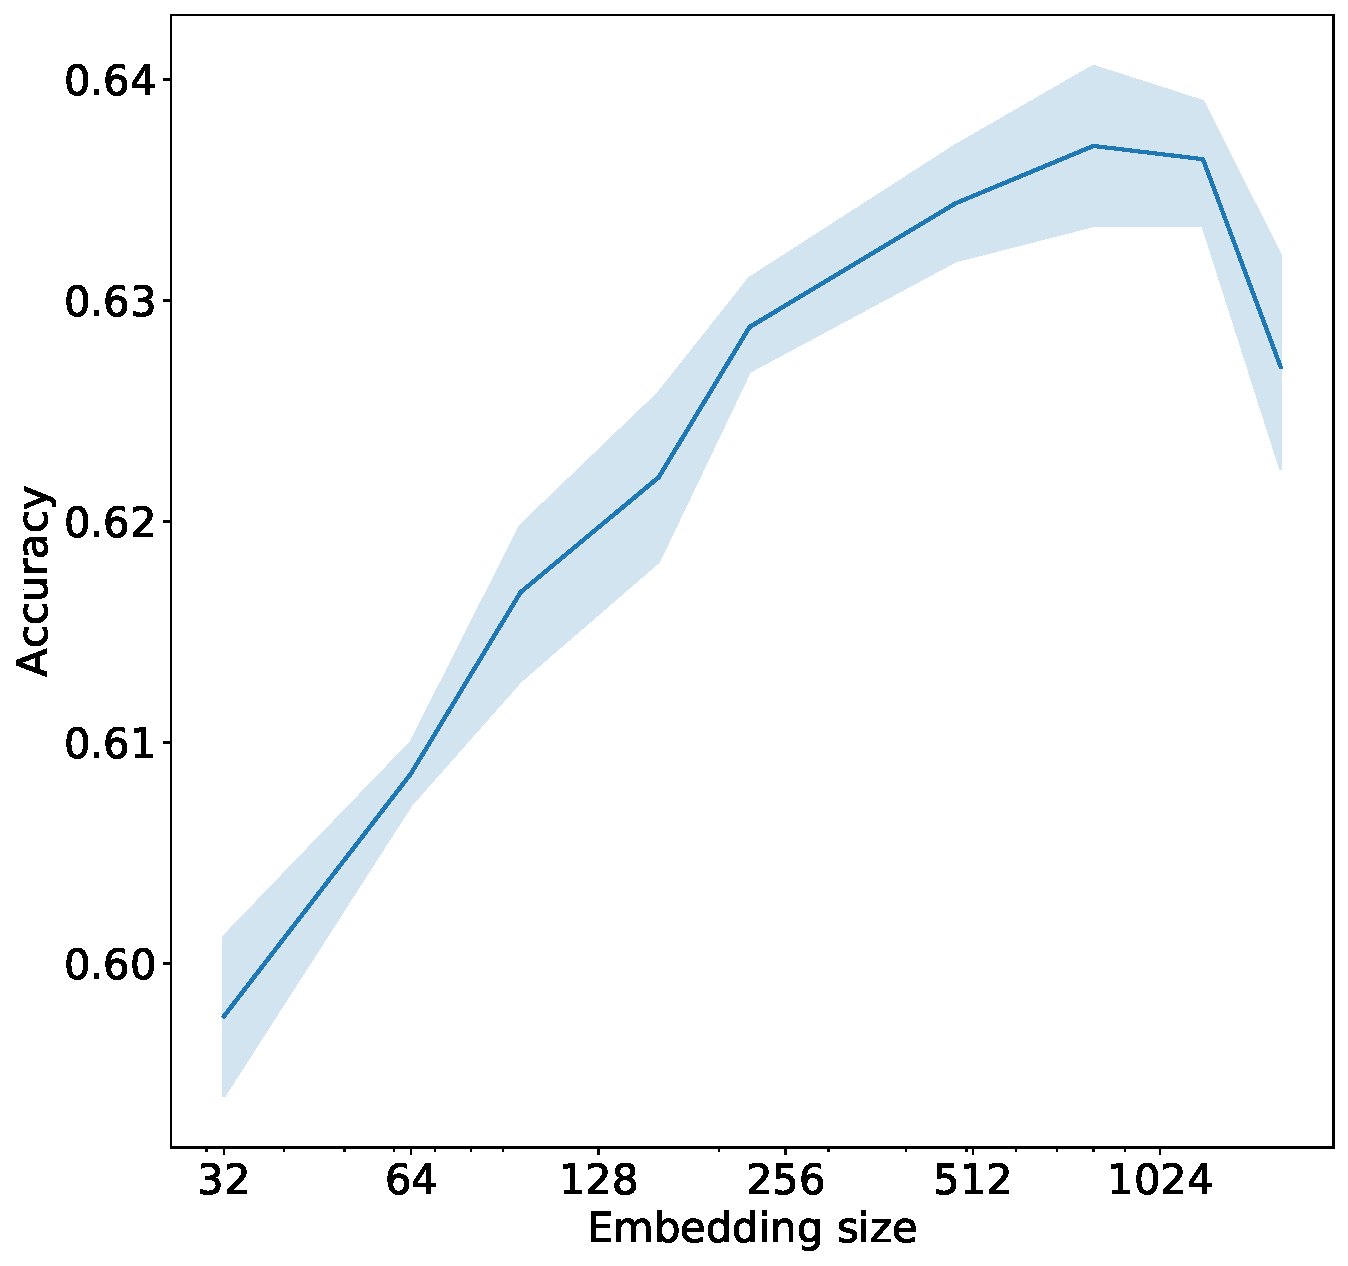
\includegraphics[width=\linewidth]{figures/age-pred-hidden-size.pdf}
    \caption{Embedding dimensionality vs. quality, age group prediction}
    \label{fig-emb-dim-age}
  \end{minipage}
  \hfill%
  \begin{minipage}[t]{0.49\linewidth}
    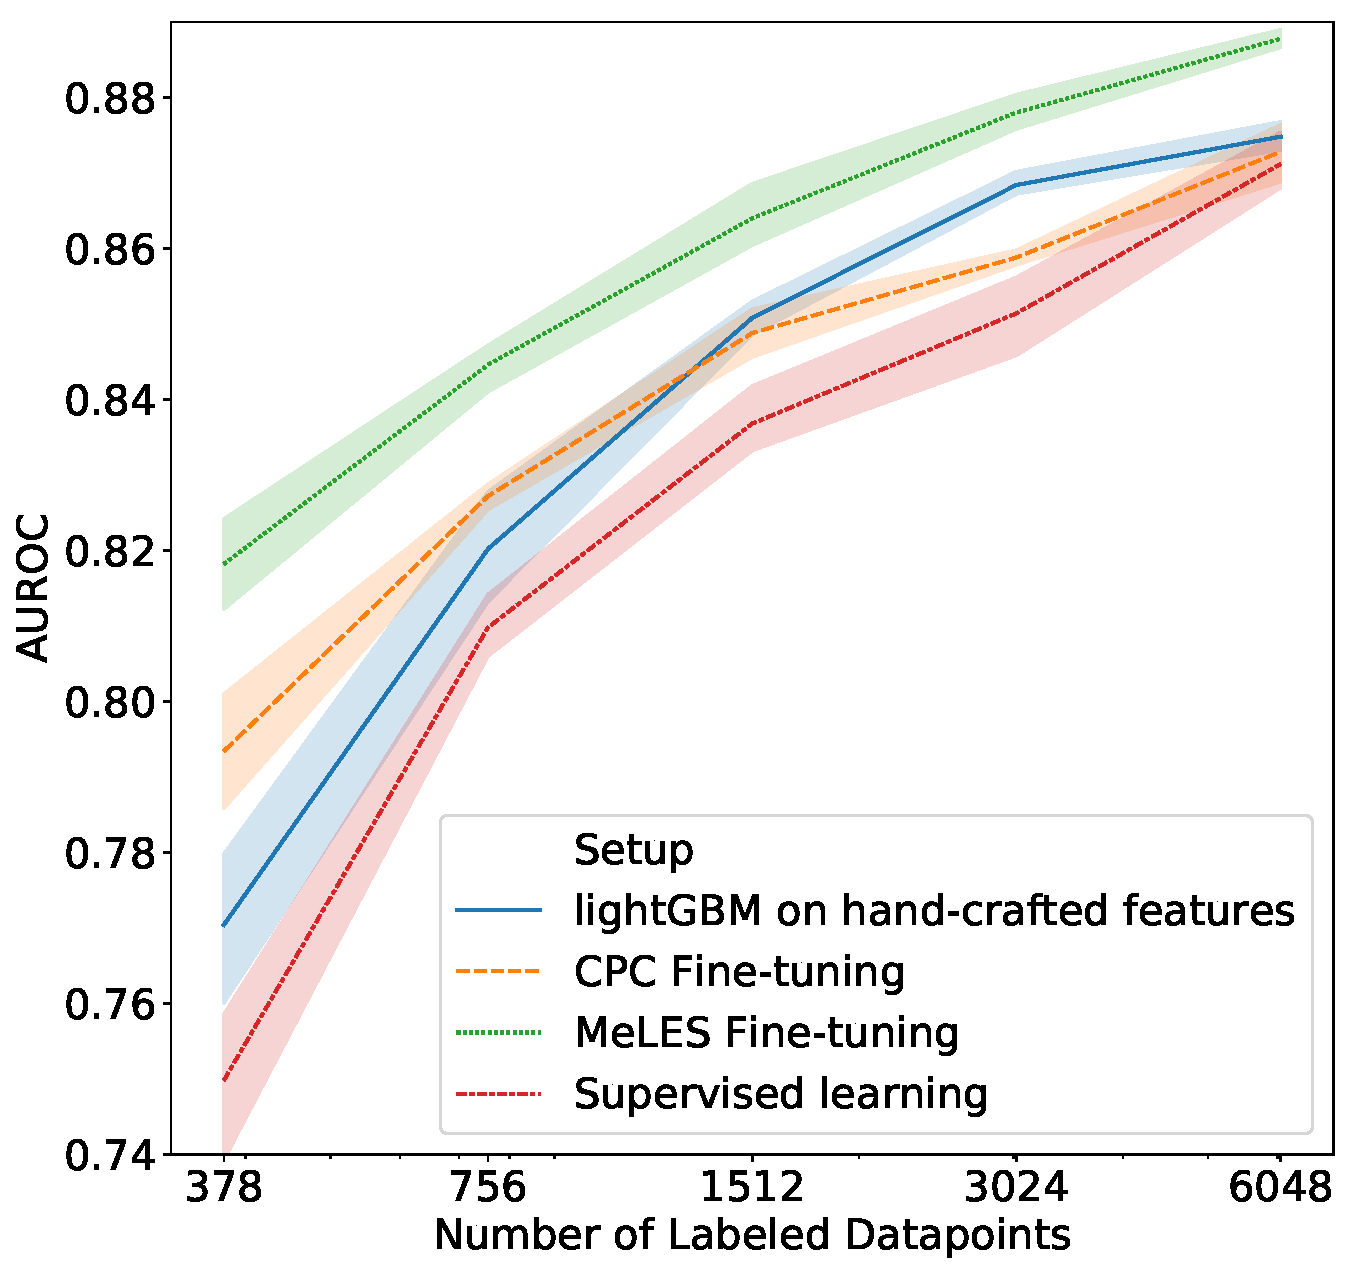
\includegraphics[width=\linewidth]{figures/ss_gen_4.pdf}
    \caption{Model quality for different dataset sizes, gender prediction}
    \small{The rightmost point correspond to all labels and supervised setup. X-axis is shown on a logarithmic scale.}
    \label{fig-semi-age}
  \end{minipage}
\end{figure}

Figure \ref{fig-emb-dim-age} shows that the quality on downstream task increases with the dimensionality of embedding. The best quality is achieved at size 800. Further increase in the dimensionality of embedding dramatically reduces quality.
The results can be interpreted as bias-variance trade-off. When embedding dimensionality is too small, too much information can be discarded (high bias). On the other hand, when embedding dimensionality is too large, too much noise is added (high variance).

In Figure \ref{fig-emb-dim-gender} we see a similar dependency. We can find a plateau between 256 and 2048, when quality on downstream tasks does not increase. The final embedding size used in the other experiments is 256.

Note, that increasing embedding size will also linearly increase the training time and the volume of consumed memory on the GPU.

\subsection{Results} \label{sec-res}

\subsubsection{Comparison with baselines} \label{sec-res-baselines}

As shown in Table \ref{tab-downstream-res} our method generates sequence embeddings of lifestream data that achieve strong performance, comparable to performance on manually crafted features when used on downstream tasks. Moreover fine-tuned representations obtained by our method achieve state-of-the-art performance on both bank transactions datasets, outperforming all previous learning methods by a significant margin.

Furthermore note that the usage of sequence embedding together with hand-crafted aggregate features leads to better performance than usage of only hand-crafted features or sequence embeddings, i.e. it is possible to combine different approaches to get even better model.

\begin{table}
\centering
\caption{Final results on the downstream tasks}
\begin{tabular}{lllll}
\toprule
\textbf{Method} & \makecell{\textbf{Age group} \\ \small{Accuracy}} & \makecell{\textbf{Gender} \\ \small{Accuracy}} &  \makecell{\textbf{Attempts} \\ \small{Accuracy}} & \makecell{\textbf{Retail} \\ \small{Accuracy}}\\
\midrule
\textbf{LightGBM on hand-crafted features} & $0.626 \pm 0.004$ & $0.790 \pm 0.008$ & $0.591 \pm 0.003$ & $0.545 \pm 0.001$ \\
\textbf{Supervised learning} & $0.631 \pm 0.010$ & $0.787 \pm 0.008$ & $0.601 \pm 0.006$  & $0.536 \pm 0.002$\\
\midrule
\textbf{LightGBM on CPC embeddings} & $0.595 \pm 0.004$ & $0.764 \pm 0.005$ & $0.584 \pm 0.004$ & $0.505 \pm 0.002$\\
\textbf{CPC fine-tuning} & $0.621 \pm 0.007$ & $0.786 \pm 0.011$ & \textbf{0.611} $\pm 0.005$ & $0.542 \pm 0.001$ \\
\midrule
\textbf{LightGBM on MeLES embeddings} & $0.639 \pm 0.006$ & $0.789 \pm 0.012$ & $0.604 \pm 0.003$ & $0.544 \pm 0.001$ \\
\textbf{MeLES fine-tuning} & \textbf{0.643} $\pm 0.007$ & \textbf{0.794} $\pm 0.005$ & \textbf{0.611} $\pm 0.005$ & \textbf{0.549} $\pm 0.001$ \\
\bottomrule
\end{tabular} \\
\small{5-fold cross-validation metric $\pm 95\%$ is shown}
\label{tab-downstream-res}
\end{table}

\subsubsection{Semi-supervised setup} \label{sec-semi}

To evaluate our method in condition of a restricted amount of labeled data we use only part of available target labels for the semi-supervised experiment.
As well as in the supervised setup we compare proposed method with ligthGBM over hand-crafted features and Contrastive Predictive Coding (see Section \ref{sec-baselines}).
For both embedding generation methods (MeLES and CPC) we evaluate both performance of the lightGBM on embeddings and performance of fine-tuned models.
In addition to this baselines we compare our method with supervised learning on the available part of the data.

In figures \ref{fig-semi-age-0} and \ref{fig-semi-gender-0} we compare the quality of hand-crafted features and embeddings by learning the lightGBM on top of them. Moreover, in figures \ref{fig-semi-age-1} and \ref{fig-semi-gender-1} one can find comparison of a single models trained on downstream tasks considered in the paper. As you can see in figures, if labeled data is limited, MeLES significantly outperforms supervised and other approaches. Also MeLES consistently outperforms CPC for different volumes of labeled data.

\section{Related work} \label{sec-rel-work}

The widely used application fields of metric learning include computer vision~\cite{Chopra2005LearningAS},~\cite{Schroff2015FaceNetAU},  NLP~\cite{Reimers2019SentenceBERTSE} and audio~\cite{Wan2018GeneralizedEL}. Conventional metric learning methods incorporate some prior knowledge of the neighborhood relationships between the training samples by the means of explicitly labelling similar and dissimilar samples.

Inspired by performance advances in pretraining on a large unlabeled dataset and fine-tuning on a smaller labeled dataset, a novel self-supervised metric learning method (SimCLR)~\cite{Chen2020ASF} related to computer vision applications has been introduced recently. SimCLR proposes visual data augmentations to construct the training samples. To the best of our knowledge, there are no self-supervised metric learning methods related to the discrete event sequence domain that have been previously proposed in the literature.

Another idea of applying self-supervised learning to non-discrete sequential data has been previously proposed in Contrastive Predictive Coding (CPC) method~\cite{Oord2018RepresentationLW}, where meaningful representations are extracted by predicting future in the latent space by using autoregressive methods. CPC representations demonstrated strong performance on four distinct domains: audio, computer vision, natural language and reinforcement learning. 

In the computer vision domain, there are many other than metric learning approaches related to self-supervised learning that are nicely summarized in~\cite{Jing2020SelfsupervisedVF}.
One of the common approaches to learn self-supervised representations is either traditional autoencoder~\cite{Rumelhart1986LearningIR} or variational autoencoder~\cite{Kingma2014AutoEncodingVB}. It is widely used for images, text and audio or aggregated event sequence data~\cite{Mancisidor2019LearningLR}. Although autoencoders have been successfully used in several domains listed above, they have not been applied to discrete event sequences either, mainly due to the challenges of defining distances between the input and the reconstructed input sequences.

\section{Conclusions} \label{sec-conclusions}

In this paper, we adopted the ideas of metric learning to the analysis of the lifestream data in a novel, self-supervised, manner. As a part of this proposal, we developed the Metric Learning for Event Sequences (MeLES) method that is based on self-supervised learning. 
In particular, the MeLES method can be used to produce embeddings of complex event sequences that can be effectively used in various downstream tasks. Also, our method can be used for pre-training in semi-supervised settings.

We also empirically demonstrate that our approach achieves strong performance results on several downstream tasks by significantly (see Section \ref{sec-res}) outperforming both classical machine learning baselines on hand-crafted features and neural network based approaches.
In the semi-supervised setting, where the number of labelled data is limited, our method demonstrates even stronger results: it outperforms supervised methods by significant margins.

The proposed method of generating embeddings is convenient for production usage since almost no pre-processing is needed for complex event streams to get their compact embeddings. The pre-calculated embeddings can be easily used for different downstream tasks without performing complex and time-consuming computations on the raw event data. For some encoder architectures, such as those presented in Section~\ref{sec-enc-arch}, it is even possible to incrementally update the already calculated embeddings when additional new lifestream data arrives.

Another advantage of using event sequence based embeddings, instead of the raw explicit event data, is that it is impossible to restore the exact input sequence from its embeddings. Therefore, the usage of embeddings leads to better privacy and data security for the end users than when working directly with the raw event data, and all this is achieved without sacrificing valuable information for downstream tasks.

\section*{Broader Impact}

Our method can be potentially used for the analysis of many different types of user activity, including online games logs, educational records, retail purchases history, internet logs and bank transactions...

% the proposed method constitutes a fair approach to credit scoring, as it does not use information about the individual and therefore cannot be used to discriminate the credit applicants by various demographic factors.

% Models on aggregate data are biased, model on raw sequiences is more fair




% Authors are required to include a statement of the broader impact of their work, including its ethical aspects and future societal consequences. 
% Authors should discuss both positive and negative outcomes, if any. For instance, authors should discuss a) who may benefit from this research, b) who may be put at disadvantage from this research, c) what are the consequences of failure of the system, and d) whether the task/method leverages biases in the data. If authors believe this is not applicable to them, authors can simply state this.

% Use unnumbered first level headings for this section, which should go at the end of the paper. {\bf Note that this section does not count towards the eight pages of content that are allowed.}

\bibliographystyle{humannat}
\bibliography{neurips2020}

\end{document}
